




\section{Method}

    \subsection{Calibration of AMOS cameras}

    we are able to isolate a small change in velocity
    and mass, which can be used directly in the numerical integration:
    \begin{equation}
        \mathrm{d}v = -\frac{\Gamma A \rho_{\mathrm{air}} v^2}{m^{1/3} \rho^{2/3}} \mathrm{d}t\text{,}
        \label{eq:mc-dv}
    \end{equation}
    
    and a change of mass due to ablation as
    \begin{equation}
        \mathrm{d}m = -\frac{\Lambda}{2Q} \frac{Am^{2/3}}{\rho^{2/3}} \rho_{\mathrm{air}} v^3 \mathrm{d}t\text{.}
        \label{eq:mc-dm}
    \end{equation}
    
    where
    \begin{description}
        \item[$\Lambda$] is a dimensionless heat transfer coefficient,
        \item[$A$] is a dimensionless coefficient of shape
    \end{description}
    
    Typical values of $\Lambda$ and $A$ are on the order of unity. The value of $\Gamma$ also depends on the properties 
    of the environment, such as viscosity or density.
    For a spherical body in a flow with Reynolds number $10^4$ a value of $\Gamma \approx num{0.47}$ is used.
    
    \cite{jones-halliday2001} defined the excitation coefficient~$\zeta$, which represents
    the sum of all excitation probabilities over collisions and obtained the following relationship between $\zeta$ and $\tau$:
    \begin{equation}
        \tau = \frac{2\epsilon\zeta}{mv^2}\text{,}
        \label{m-tau}
    \end{equation}

    where $\epsilon$ is the mean excitation energy. For estimation of $\zeta$ we used a slightly improved version of the
    model compiled by \cite{hill2005}. In the formulae speed $v$ is stated in metres per second.
    To obtain the total flux of emitted visible light $F_0$, we take the time derivative of the particle's kinetic energy.
    Neglecting the second (deceleration) term yields the following \emph{equation of luminance}:
    \begin{equation}
        F_0 = \tau(v) \frac{\Lambda}{4Q} \rho_{\mathrm{air}} v^5\text{.}
        \label{m-f0}
    \end{equation}

    With this knowledge we are able to calculate the total luminous power of the meteor and subsequently its absolute magnitude.

\section{Simulation}
    
    \subsection{Generating the population}
    spherical earth
    
    \subsection{Observations}
    

\section{Physics of meteor flight} \label{sim:pmf}
    The analysis begins with detailed understanding of the physics of meteor flight in the upper atmosphere.
    /
    However, the used model needs to be reasonably simple and only replaced by a more 
    once there is an obvious reason to do so.
    
    \subsection{Equations of motion}            
        We use the standard model of meteor atmospheric flight developed by \cite{opik1958}.
        
        Since the simulation is primarily used to simulate small particles that ablate completely in the atmosphere,
        we do not need to account for meteoroid fragmentation 
        
        Hence, we only assume spherical particles
    
        \subsubsection{Braking equation} \label{sim:pmf:em:be}
            While atmosphere exerts a multitude of forces on the entering meteoroid particle,
            they are dominated by the drag force, acting in the direction opposite to the meteoroid's velocity vector.

            For small bodies at high velocities the influence of the Earth's gravity is negligible, 
            as they burn completely in a very short time. Forces with components perpendicular
            to the direction of the flight, such as aerodynamic lift or rocket effect caused by outgassing,
            can also be ignored. These assumptions are justified as long as we constrain the simulation to small particles which
            do not survive the atmospheric entry, and only consider entry speeds greater than the
            escape speed at any given altitude. Both conditions hold very well for meteoroid particles observed by
            intensified CCD cameras.

            Thus, for the purpose of the simulation we assume that each meteoroid particle always moves in a straight line
            and is only subject to deceleration caused by aerodynamic drag. We consider the standard form of the
            aerodynamic drag equation:
            \begin{equation}
                ma \equiv m\dot{v} = -\Gamma S \rho_{\mathrm{air}} v^2\text{,}
                \label{sim:pmf:em:be:ma}
            \end{equation}

            where
            \begin{itemize}
                \item $m$ is the instantaneous mass of the meteoroid particle (\si{\kilo\gram}),
                \item $\Gamma$ is the drag coefficient (dimensionless),
                \item $S$ is the cross-sectional area of the particle in the plane perpendicular to its velocity vector (\si{\metre\squared}),
                \item $v$ is its speed relative to the surrounding medium (\si{\metre\per\second}).
            \end{itemize}

            Note that while $\Gamma$ represents the shape of the particle, it is not constant during the flight.
            It also depends on the properties of the particle's surface, its attitude and various properties of the environment,
            such as Reynolds number (the ratio of inertial and viscous forces acting on the fluid surrounding the particle),
            air density and pressure. Its typical values are on the order of unity.
            $\Gamma \approx \num{0.47}$ corresponds to a spherical body in a flow with Reynolds number $10^4$.
            Values between \num{0.4} and \num{0.8} are typical for real meteoroid particles.

            We may express $S$ in terms of a dimensionless \emph{coefficient of shape} $A$, which is independent of the size of the particle;
            mass of the particle $m$ and its (constant) density $\rho$. This means that explicitly calculating the cross-sectional
            area is no longer necessary during the simulation.
            \begin{equation}
                S = A V^{2/3} = \frac{A m^{2/3}}{\rho^{2/3}}\text{,}
                \label{sim:pmf:be:S}
            \end{equation}

            where $V$ denotes the particle's volume. After dividing by $m$, equation \ref{sim:pmf:be:ma} takes the form
            \begin{equation}
                \mathrm{d}v = - \frac{\Gamma A}{m^{1/3}\rho^{2/3}}\rho_{\mathrm{air}} v^2\text{.}
                \label{sim:pmf:be:dotv}
            \end{equation}

            If the atmosphere is calm, $v$ is always equal to the magnitude of the particle's geocentric velocity $\vec{v}$.
            With meteors this assumption is well justified, since $v_{\mathrm{air}} \ll v$.
            Finally, for the purposes of the integrator a small change of velocity $\mathrm{d}v$ can be isolated:
            \begin{equation}
                \mathrm{d}v = -\frac{\Gamma A \rho_{\mathrm{air}} v^2}{m^{1/3} \rho^{2/3}} \mathrm{d}t\text{.}
                \label{sim:pmf:be:dv}
            \end{equation}

        \subsubsection{Equation of ablation} \label{sim:pmf:ea}
            In the model we assume that all of the available kinetic energy is converted to thermal energy and used
            to evaporate the material of the particle. This approximation is justified as long as the specific heat
            of vaporization is much greater than the thermal capacity of surrounding air. The equation takes the form
            \begin{equation}
                \dot{m} = -\frac{\Lambda}{2Q} S \rho_{\mathrm{air}} v^3\text{,}
                \label{sim:pmf:ea:dotm}
            \end{equation}

            where
            \begin{itemize}
                \item $\Lambda$ is the heat transfer coefficient (dimensionless);
                \item $Q$ is the specific enthalpy of vaporisation of meteoroid material
                    ($\si{\joule\per\kilo\gram} \equiv \si{\metre\squared\per\second\squared}$).
            \end{itemize}

            In real objects most of these quantities vary wildly on scales far smaller than the typical dimension of the particle.
            Naturally, such precision is meaningless in the simulation, so only constant values are considered. Either fixed mean values
            are used for the entire simulation, or each new particle is assigned a value randomly drawn from
            a pre-defined probability distribution. This is particularly important when generating particle masses.

            Once again, for the numerical simulation we need to isolate the change of mass $\mathrm{d}m$
            in a small time interval $\mathrm{d}t$:
            \begin{equation}
                \mathrm{d}m = -\frac{\Lambda}{2Q} \frac{Am^{2/3}}{\rho^{2/3}} \rho_{\mathrm{air}} v^3 \mathrm{d}t\text{.}
                \label{sim:pmf:ea:dm2}
            \end{equation}

        \subsubsection{Equation of luminance} \label{sim:pmf:el}
            In order to determine the apparent brightness of a simulated meteor, its absolute brightness must be calculated first.
            For the sake of simplicity we assume a constant fraction of total released energy is emitted as visible light,
            as opposed to energy lost to the atmosphere or consumed in heating and evaporating the body:
            \begin{equation}
                \Phi_e \propto \frac{\mathrm{d}E_\mathrm{kin}}{\mathrm{d}t}\text{.}
                \label{sim:eq:lum:dekin}
            \end{equation}

            where $\Phi_e$ denotes the total isotropic \emph{radiant flux} over all visible wavelengths of the elecromagnetic spectrum.

            The constant of proportionality is usually denoted $\tau$ and named \emph{luminous efficiency factor} \cite{hill2005}.
            Most of the particle's kinetic energy is transformed
            to heat and ionization of atoms and only a very small fraction is emitted as visible light.
            Luminous efficiency is usually considered to be a function of speed and
            meteoroid material \cite{jones-halliday2001}. Since we assume a homogeneous composition for each meteoroid,
            in each flight simulation $\tau$ is solely a function of speed and as such must be recomputed in every integration step.
            Its typical values are on the order of $10^{-2}$.

    \subsection{Supplementary quantities} \label{s}
        In addition to the properties of the meteoroid particle itself, the simulator needs to know various
        properties of the environment or the observer.

        \subsubsection{Atmospheric density}
            The density of the air $\rho_{\mathrm{air}}$ appears in all of the above equations
            and must be calculated before any equations of motion can be solved.
            At the altitudes where meteors occur the standard isothermal approximation no longer holds.\footnote{At \SI{100}{\kilo\metre},
            isothermal atmosphere overestimates density by a whole order of magnitude compared to the output of
            a high-precision model \cite{msise90}.} Therefore it is necessary to use a more precise model.
            
            High-order polynomial fitting atmospheric models, such as those found in \cite{braeunig2014} and \cite{ussa1976}, are sufficiently precise,
            however, since air density must be calculated in every iteration of the integrator, their use is prohibitively expensive.

            In order to reduce computation time we used a simple and fast tabular approximation of the
            NASA Mass-Spectrometer-Incoherent-Scatter Extended 1990 (MSIS-E-90) atmosphere model \cite{msise90}.
            Values were tabulated by \SI{1}{\kilo\metre} and interpolated by a piecewise exponential function.
            The results of this approximation differ from true values in the model less than one part in ten thousand,
            which greatly exceeds the required precision.

        \subsubsection{Air mass} \label{sim:pmf:sq:am}
            Air mass calculation is crucial for determining the effects of atmospheric extinction.
            It is perfectly reasonable to use the same function as in \ref{fwd:nbs:opt:ae}.
            Since magnitude scale is logarithmic in nature and the decrease in brightness in exponential,
            the resulting increase in apparent magnitude is linearly proportional to optical thickness, which is in turn
            linearly proportional to air mass.

        \subsubsection{Coordinate transformations} \label{sim:pmf:sq:ct}
            To achieve highest precision \textsc{Astropy}'s built-in \texttt{EarthLocation} class should be used.
            The positions are internally represented as three-dimensional Cartesian vectors. Human-readable output
            and altitude calculations are obtained after transforming the coordinates to \texttt{WGS84} geoid.

            However, computation time can be drastically reduced if the Earth is modelled as a sphere. Since
            flattening of the Earth spheroid is only approximately $1/298$ \cite{nima2000}, this approximation does not
            result in significant errors compared to other simplifications we have already made.
            It should be noted that the error also depends on the distance between the meteor and the observer,
            which is always much less than the radius of the Earth; and the total error is thus negligible.

        \subsubsection{Angular speed} \label{sim:pmf:sq:as}
            The calculation of perceived brightness also requires taking angular speed into account.
            Light from faster meteors is spread on a larger number of CCD pixels,
            lowering the signal-to-noise ratio and thus also the probability of a successful detection.

            In context of meteor motion, angular speed means the apparent length of the projection of the meteor's
            true velocity vector onto the celestial sphere.
            Let us denote this vector $\vec{v}$ and let $\vec{r}$ be the position of the meteoroid with respect to the observer.
            The projection onto a spherical sky can be represented as the projection onto a plane perpendicular to $\vec{r}$ and
            passing through the meteoroid, which we will denote $\mathrm{rej}_{\vec{r}}\vec{v}$.%
            \footnote{The projection of $\vec{v}$ onto the plane perpendicular to $\vec{r}$ is also called the \emph{rejection}
            of $\vec{v}$ onto $\vec{r}$ \cite{perwass2008}.}
            
            For any two vectors $\vec{r}$ and $\vec{v}$, $\vec{v}$ is the sum of its projection and rejection onto $\vec{r}$:
            \begin{equation}
                \mathrm{proj}_{\vec{r}}\vec{v} + \mathrm{rej}_{\vec{r}}\vec{v} = \vec{v}\text{.}
                \label{sim:pmf:sq:as:rej}
            \end{equation}
            
            The projection vector can be obtained easily using dot product as
            \begin{equation}
                \mathrm{proj}_{\vec{r}}\vec{v} = \frac{\vec{r}\cdot\vec{v}}{r} \cdot \frac{\vec{r}}{r} = \frac{\vec{r}\cdot\vec{v}}{r^2}\vec{r}\text{.}            
                \label{sim:pmf:sq:as:proj}
            \end{equation}
            
            Putting these equations together we obtain the formula for apparent angular speed,
            \begin{equation}
                \omega = \frac{\left|\vec{v} - \frac{\vec{r}\cdot\vec{v}}{r^2}\vec{r}\right|}{r}\text{.}
                \label{sim:pmf:sq:as:asf}
            \end{equation}

\section{Algorithm}
    With full knowledge of underlying equations, we may proceed to designing the simulation algorithm.

    \subsection{Generating the meteoroids}
        The first step of the simulation is to create the initial population of meteoroid particles entering the atmosphere.
        At this point, we pretend not to know anything about observers and are only concerned with
        physical representations of virtual meteoroid objects.
        
        To reduce the size of the possible parameter space, we fixed the values of most
        parameters that are known CITE THIS or can be determined experimentally, such as the        
        \begin{itemize}
            \item heat transfer coefficient $\lambda$ (\num{0.5}),
            \item specific heat of vaporizarion $Q$ (\SI{8}{\mega\joule\per\kilo\gram}),
            \item coefficient of shape (\num{0.47}).
        \end{itemize}

        In \textsc{Asmodeus}, this process in handled by the script \texttt{asmodeus-generate.py}.
        
        \subsubsection{Initial masses}
            First of all the particles are assigned their initial mass. Meteor showers are typically described
            by the \textbf{mass population index} $s$. The differential spectrum of masses follows a power law:
            \begin{equation}
                N(m) = m^{-s}\text{,}
            \end{equation}
            
            with typical values of $s$ being \numrange{1.5}{2.5}. Since this distribution is divergent for $m \to 0$,
            we also need to establish the lower bound on meteor masses $m_\mathrm{min}$. This requirement effectively yields
            a Pareto I distribution with $s$ as the parameter of scale and $m_\mathrm{min}$ as the XXXXXXX.
            
            have a look at this again
            
        \subsubsection{Initial positions}
            Each meteoroid particle is assigned a starting position within a predefined geographic area. Its precise bounds
            are not important and may be chosen somewhat arbitrarily, as long as several conditions hold:        
            \begin{itemize}
                \item The entire sky visible from each station must be covered. Setting the bounds too close to the observers
                    will result in less generated meteors in that direction, especially near the horizon. This would
                    introduce undesirable skewing to the observed distribution.
                \item The total area should be as small as possible. If the area is too large, most meteors will be never registered
                    after atmospheric extinction and other effects are applied, while the required computation time
                    stays roughly the same as with registered meteors.
                \item The shape of the area should be simple. Sampling the source distribution should be a straightforward process.
            \end{itemize}
        
            Setting an artificial limit on the statistics, for instance requiring the altitude to be at least \ang{15},
            simplifies fulfilling these conditions significantly. The minimum required area is also easier to calculate this way.

            Two simplest shapes are a spherical rectangle\footnote{By this we mean a true \emph{rectangle}, ie. a figure with four right angles,
            bounded by two parallels and two meridians. ``Spherical rectangle'' usually refers to a shape whose
            four angles are equal, but necessarily larger than \ang{90}.} and a circle.
            A slight disadvantage of the rectangle is that the distribution cannot be sampled as two independent
            uniform distributions, since this would result in more meteoroids being generated at the side closer to the pole.

            This excess can be described in terms of geographic latitude $\phi$. On a spherical Earth
            the length of a parallel is equal to $R \cos{\phi}$: if meteoroid longitudes are sampled
            from a uniform distribution, the excess will be proportional to $\frac{1}{\cos\phi}$.
            
            To correct the distribution and obtain a constant particle density of the entire covered part
            of the surface, we might discard the excess meteoroids immediately. This can be achieved simply
            by only accepting particles with probability $p_a$, proportional to the length of th intersection
            of the parallel where the meteoroid was placed upon generation:
            \begin{equation}
                p_a(\phi) = \cos\phi\text{.}
                \label{sim:al:gtm:ip:proba}
            \end{equation}
            
            A slight performance increase can be achieved by normalizing the density to the
            length of the parallel closest to the equator. All meteoroids generated at this boundary will be accepted,
            resulting in less wasted computation time.
            Equation \ref{sim:al:gtm:ip:proba} then transforms to
            \begin{equation}
                p_a(\phi) = \frac{\cos\phi}{\cos\phi_0}\text{,}
                \label{sim:al:gtm:ip:prob2}
            \end{equation}

            where $\phi_0$ is the latitude of the parallel closest to the equator.
            
            For meteor showers we also need to include the effects of the altitude of the radiant.
            Higher altitudes (or conversely, lower zenith distances) result in a larger effective projection area.
            The effect is proportional to the sine of the radiant altitude.
            
            Once again, we may solve this by accepting generated meteors with a certain probability $p_r$,
            which varies with altitude of the radiant at the time of the atmospheric entry at
            the position of the meteor above the Earth's surface.
            Of course, it must be computed for each meteor independently.
            \begin{equation}
                p_r = \cos\theta_r(\phi, \lambda, t)\text{,} 
                \label{sim:al:gtm:ip:probr}
            \end{equation}
            
            where
            \begin{itemize}
                \item $\theta_r$ is the altitude of the radiant,
                \item $\phi$ is the latitude of the meteoroid particle,
                \item $\lambda$ is the longitude of the meteoroid particle,
                \item and $t$ is the time of the entry.
            \end{itemize}
            
            The probability that a generated meteoroid will be accepted and simulated
            is determined by the product of probabilities \ref{sim:al:gtm:ip:prob2} and \ref{sim:al:gtm:ip:probr}.           
           

        \subsubsection{Initial velocities} \label{sim:al:gm:iv}
            In the next step we need to assign the particles their initial velocities.
            There are two distinct approaches to this problem, depending on whether
            the program simulates a particular \emph{meteor shower} or the \emph{sporadic background}.
            
            Simulating the sporadic background would be significantly more challenging. The apex, antapex and anthelion
            sources present different flux densities, which change with time and location.
            With meteor showers the situation is substantially simpler: all particles share a common parent
            body, which translates to a common radiant and similar atmospheric entry speeds.
            On the contrary, sporadic background exhibits a relatively constant average flux,
            while intensities of meteor showers vary considerably even on short time scales.
            
            Naturally, the real observed distribution includes both sources simultaneously.
            In the simulation we only considered meteor showers with constant radiant
            with respect to the geocentric equatorial coordinate system.
            The transformation to an ECEF\footnote{Earth-centered, Earth-fixed -- a terrestrial coordinate system, rotating with the Earth,
            as opposed to a nonrotating celestial coordinate system} coordinate system is fairly straightforward
            and already implemented in \textsc{Astropy}.
                        
            Note that while initial velocities of the particles in the simulation are not equal to their true geocentric velocities,
            as would be observed outside the gravitational influence of the Earth.
            
            Simulations of sporadic background meteors are also planned once the system is tested.

        \subsubsection{Atmospheric entry}
            Once the initial position is deemed acceptable, atmospheric entry may be simulated and recorded.            
            In \ref{sim:pmf} we obtained a system of interdependent differential equations,
            which can be solved numerically.
            
            Two solver have been evaluated. The semi-implicit Euler integrator is much easier to
            implement and requires significantly less time to evaluate one step, but requires a large number
            of steps to achieve sufficient precision.

            A fourth-order Runge-Kutta solver is more precise but also more difficult to implement,
            especially since the mass of the meteoroid is changing during the simulation.
            Considerable effort has been made to ensure the solver produces correct results.
            
            The frequency of the captured frames is equal to the frame rate of real AMOS cameras.
            In Slovakia, the frame rate is fixed at 15 frames per second.            
            This does not necessarily equal the time step taken by the integrators,
            as multiple small steps may be taken between two successive frames.
            The interpolating steps are discarded and only 15 frames per second
            are selected for further analysis.
            
            In practice, we found that the precision of RK4 integrator does not
            increase noticeably if time step is set to less than 1/75 of a second
            while computation time is still acceptable. 
            
            If higher precision
            
    \subsection{Processing the observations} \label{sim:al:po}
        In the next step each meteoroid is \emph{observed} -- its projection on the sky
        is computed for each of the observing stations, along with its apparent luminosity
        and other important properties as observed in each frame.
        
        \subsubsection{Calculation of projection}
            Meteor projections are computed independently for each observer.
            The geographic coordinates are first transformed to an observer-centered altitude-azimuthal coordinate system.
            As a spherical Earth model is used, this is done easily by several matrix transforms.            
            AMOS cameras project the sky in an equidistant polar projection: each degree of altitude is
            transformed to an equal radial distance on the CCD. This simplifies plotting
            the observed meteors, as a 2D polar chart may be used without any further adjustments.
            
            To establish the apparent brightness, luminous flux at the location of the observer is calculated.
            The total luminous power in each frame is reduced to the surface of a sphere with radius equal
            to the distance between the frame and the observer to obtain luminous flux in watts per square metre:
            \begin{equation}
                I \propto d^{-2}\text{.}
                \label{sim:al:po:cp:d}
            \end{equation}
            
            This value is further reduced by atmospheric extinction. Extinction is described in terms of \textbf{relative air mass} $X$,
            which is a dimensionless quantity that specifies the ratio of optical thickness in the direction of the observed
            object to the optical thickness in zenith:
            \begin{equation}
                X = \frac{%
                    \int\limits_{\text{observer}}^{\text{zenith}} \kappa(s)\rho_{\mathrm{air}}(s) \mathrm{d}s%
                }{%
                    \int\limits_{\text{observer}}^{\text{object}} \kappa(s)\rho_{\mathrm{air}}(s) \mathrm{d}s%
                }\text{.}
                \label{sim:al:po:cp:airmass}
            \end{equation}
            
            High precision air mass models have been developed, such as \cite{kasten-young1989}.
            The decrease in brightness increases exponentially with optical thickness as $e^{-kX}$ for some constant $k$.
            This constant must be determined experimentally. If we assume that the atmospheric effects make
            a meteor in zenith $(X = 1)$ appear about \SI{25}{\percent} dimmer, $k$ must be equal to
            $-\ln \left(1 - 0.2\right) \approx 0.288$.
            
        \subsubsection{Application of selection bias}
            After all natural effects have been applied and apparent position and magnitude have been computed,
            we need to simulate the instrumental effects, introduced by the detection apparatus.
            
            Various sources of selection bias 
            For further details refer to \cite{balaz-inprep}.
            
            We assumed a sigmoid profile of the detection efficiency curve:
            \begin{equation}
                D(m) = \frac{f}{1 + e^{\frac{m - m_0}{\omega}}}\text{.}
                \label{eq:sls}
            \end{equation}
            
            where
            \begin{itemize}
                \item $m_0$ is the limiting magnitude, defined as the point where
                    detection efficiency is equal to half of its maximal value.
                \item $\omega$ denotes the width of the distribution.
                    Smaller values correspond to a sharp detection efficiency falloff.
                \item $f$ is the \emph{fill factor}: the upper limit of the system's detection ability.
                    Random occurrences, such as discriminator failures, power outages and similar problems
                    may prevent detection even under otherwise perfect conditions. Thus even for very
                    bright bolides detection is not always assured.
            \end{itemize}

            The exact shape of the detection efficiency profile was derived from observational data.
            In the dimmer part of the apparent luminosity spectrum ($-2^\mathrm{m}$--$5^\mathrm{m}$),
            two nights of simultaneous observations by two AMOS cameras and seven human observers were analyzed.
            Only meteors captured by human observers were taken into account. We investigated all visual meteor records
            and paired them with automated records by timestamps. The fraction of meteors captured by AMOS
            was recorded 
            
            These data did not include any meteors brighter than $-2^{\mathrm{m}}$.           
            Bolide data were obtained from long-term simultaneous observations with AMOS cameras and photographic
            plates at AGO Modra. We asserted that the photographic plate is a perfect observer and searched for corresponding
            records in AMOS databases. Again, we ignored all AMOS reports of bolides that were not captured on photographic plates.
            The data were collected at AGO Modra between 2010 and 2016. AMOS registered 57 out of 67 bolides recorded on
            the plates.

            After putting both data sources together we fitted the observed distribution with function \ref{sim:al:po:asb:dm}.
            
            \begin{figure}
                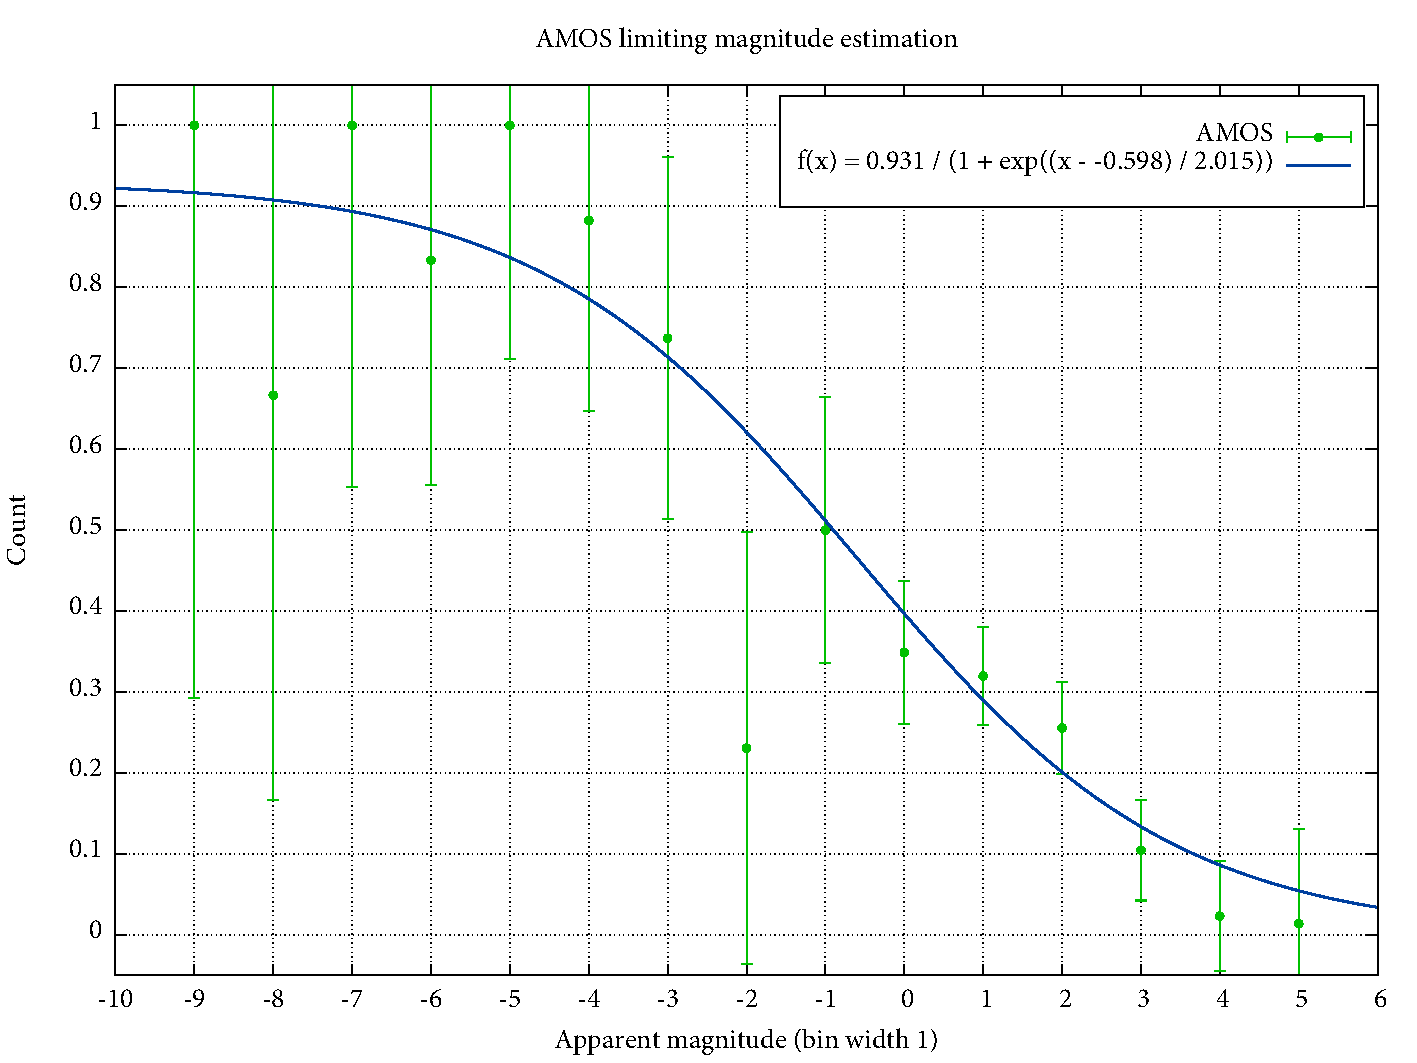
\includegraphics[width = \linewidth]{pictures/limmag.pdf}
                \caption{Detection efficiency falloff curve.
                    Bin width $1^\mathrm{m}$, error bar size is $\frac{1}{\sqrt{N + 1}}$, where $N$ is the number of observed meteors in the bin.
                    Limiting magnitude is $\mu \doteq \num{-0.6}$, falloff rate is $\omega \doteq \num{2}$, and fill factor reaches
                    over \SI{93}{\percent}.
                }
                \label{sim:al:po:limmag}
            \end{figure}

\section{\textsc{Asmodeus}}
    The described algorithm has been implemented and tested in a suite of scripts named \textsc{Asmodeus}.
    The name is a free acronym of \textbf{A}ll-\textbf{s}ky \textbf{M}eteor \textbf{O}ptical
    \textbf{D}etection \textbf{E}fficiency \textbf{S}im\textbf{u}lator.
    \textsc{Asmodeus} is written in Python 3 and uses the \textsc{Astropy} library.

    \subsection{Operation} \label{sim:op}
        First, configuration data are loaded from the specified file in \texttt{YAML} format.
        Certain parameters may be overridden using command-line arguments.

        \texttt{N} meteors are then simulated. Each meteor is assigned a starting position within predefined
        geographic coordinates at a fixed altitude of \SI{150}{\kilo\metre}, and a geocentric velocity vector.
        Positions are sampled from a uniform distribution. For a meteor shower, the velocity vector components
        are constant in the equatorial coordinate system.

